This chapter will describe three control rod decusping methods developed as part of this work.  The first method is polynomial decusping, a simple correction based on pregenerated data.  The second method is subplane collision probabilities.  This method extends the subplane scheme by introducing a 1D collision probabilities calculation to capture subgrid information around partially inserted rods.  The final method presented here is the subray method of characteristics.  This modified form of MOC directly accounts for the partially inserted rod in the 2D MOC calculations instead of applying corrections to cross sections afterwards.

\section{Polynomial Decusping}

The polynomial decusping technique was developed to provide a fast, simple correction to the cusping problem in the MPACT code.  This technique assumes that the reactivity and power around the partially inserted rod have a predictable shape as functions of the rod position within the MOC plane.  Based on this assumption, correction factors were developed to reduce the volume fraction of control rod material and reduce the magnitude of the cusping effects.

To do this, a 3$\times$3 assembly problem with a control rod in the center assembly was used (this problem is described in more detail in Section \hl{number}).  

\section{Subplane Collision Probabilities}

The subplane scheme as it was originally conceived was used primarily to address stability issues caused by thin MOC planes in early 2D/1D codes.  While other improvements to the 2D/1D method have largely eliminated these problems, the idea of capturing subplane information using the subplane scheme can be useful for addressing partially inserted rods without substantially increasing the computational cost.  To do this, three changes were made to the basic subplane scheme: an axial correction, a radial correction, and an MOC cross section correction.

\subsection{Axial Correction}

Traditionally, the subplane scheme uses axially constant cross sections for all subplanes in each MOC plane.  When a control rod is partially inserted in the plane, a flux-volume homogenized cross section is calculated and used for each subplane.  This allows the subplane scheme to be used, but does little to account for the partially inserted rod.

To resolve this issue, the subplanes with the control rod use the rod cross section, and the subplane without the rod use the moderator cross section.  These cross sections are still homogenized using flux-volume weighting as before, but without homogenizing axially.  Doing this allows both the CMFD and P$_3$ calculations to capture some of axial effects of the partially inserted rod, reducing the magnitude of the cusping errors around the rod.

\subsection{Radial Correction}

Using axially heterogeneous cross sections within an MOC plane corrects some of the cusping effects, but it does not accurately capture the radial effects of the partially inserted rod.  In reality, the radial flux shape in the rodded subplanes is completely different from the shape in the unrodded subplanes.  The MOC calculations are done on the thicker MOC planes using axially homogenized cross sections in the partially rodded regions.  This produces a radial flux shape that is not representative of either the rodded or unrodded region, as illustrated in figure \hl{number}.  Thus, using this radial flux shape to calculate the pin-homogenized cross sections for CMFD P$_3$ introduces some error in the cross sections.

\begin{figure}
    \centering
    \caption{Radial flux shapes for rodded, unrodded, and axially homogenized MOC pin cells}\label{f:radialFluxProfiles}
\end{figure}

To account for this, a 1D collision probabilities calculation is introduced during the homogenization step.  These calculations are done in the rodded and unrodded regions to generate separate radial flux shapes that can be used during the CMFD homogenization step, as shown in Figure \ref{f:SCPdecusping}.  These CP calculations are done for each energy group and consist of inverting a small $N_r \times N_r$ matrix, where $N_r$ is the number of rings in the pin cell model (usually less than 10).  Because these matrices are so small, these calculations are computationally negligible when compared with the full 2D/1D iteration scheme while providing more accurate radial information for the cross section homogenization.

\begin{figure}
    \centering
    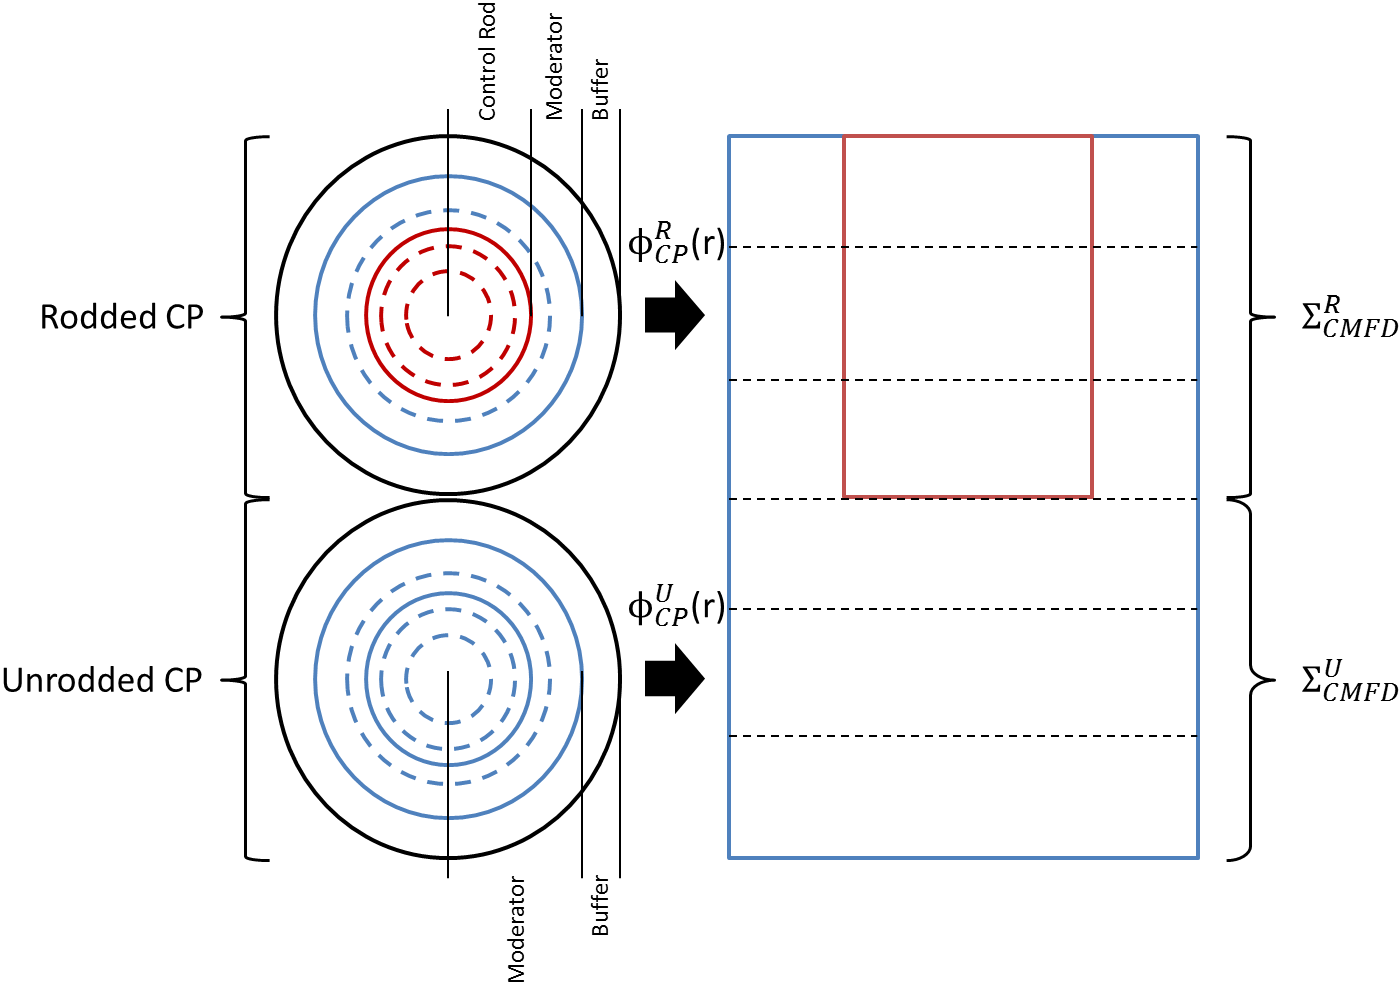
\includegraphics[width=0.8\textwidth]{CPdecusp.png}
    \caption{Illustration of subplane collision probabilities used on a partially inserted rod}\label{f:SCPdecusping}
\end{figure}

\subsection{MOC Correction}

The final step in this decusping technique is to use the subplane information from the CMFD/P$_3$ calculations to improve the MOC calculations.  To do this, the volume-homogenized cross sections are updated each iteration using a flux-volume weighting that involves the axial flux shape from the CMFD/P$_3$ system and the radial flux shape from the CP calculations.  These are combined the same was as the nTRACER method using Equation \ref{e:nTRACERdecusping}.

\section{Subray Method of Characteristics}

The previous two methods are each effective in reducing the effects of rod cusping, as will be shown in Chapter \hl{number}.  Despite these improvements, each method has significant drawbacks:
\begin{itemize}[leftmargin=*]
    \item \textbf{Polynomial Decusping}
    
    \begin{itemize}
        \item Corrections are limited to certain control rod materials (AIC, B$_4$C, Tungsten).
        \item Limited accuracy, especially for problems significantly different from those used to generate data.
    \end{itemize}

    \item \textbf{Subplane Collision Probabilities}
    
    \begin{itemize}
        \item CP is limited to TCP$_0$ scattering.
        \item CP implementation for non-cylindrical geometries can be complicated (e.g., BWR control blades).
        \item Instability can be introduced in the CP calculations by large transport corrections.
        \item MOC calculations are still performed using homogenized cross sections.
    \end{itemize}
\end{itemize}
The most important inaccuracy in the subplane CP method is the final point.  To fully address the partially inserted rod, it is desirable to account for the rod in the 2D MOC calculations themselves using heterogeneous cross sections.  Doing so will greatly improve the overall accuracy of the 2D/1D calculation by improving the accuracy of the transport itself.

\subsection{1D MOC Code and Problem Description}

To develop this new method, a 1D MOC code was developed to investigate the behavior of angular and scalar flux near a partially inserted control rod.  This code was written in Matlab \hl{citation?} and is set up to take in a description of pins and materials to be used for the calculations.  For the geometry, a pin pitch is specified which is used for all pins.  Each pin consists of a list of radii.  Assuming a square pin cell, these pins are then transformed from cylindrical geometry to slab geometry while preserving the volume fraction of each material.  Thus, the thickness of the pin slab is equal to the pin pitch, but the width of the fuel material will not be equal to input radius, since the volume fractions are preserved.  This transormation can be done assuming along one of two directions: side-to-side through the center of the square pin cell or corner-to-corner, allowing the two extremes of azimuthal angles to be considered.

Each region in the problem is divided into subregions to ensure the solution is mesh-converged.  Each region is then assigned a material from a cross section library file.  This file uses the ``user library'' format supported by MPACT, which allows the user to input macroscopic cross-sections for absorption, nu-fission, kappa-fission, chi, and scattering moments.  For all these calculations, the C5G7 benchmark cross-sections \cite{EELewisC5G72003,EELewisC5G7extended2005} were used.  These cross sections are included in Appendix \ref{app:c5g7xs}.

For the MOC sweeps, a Gaussian quadrature \cite{HandbookOfMathFunctions1972} is used with 2, 4, 8, 16, or 32 polar angles, with half of the angles being used in each direction.  The MOC sweeps are done similarly to how they are done in MPACT, with the loop over energy groups being the innermost loop.  The code can be run as either a fixed source solver or an eigenvalue solver.  For the eigenvalue mode, power iteration is used after each MOC calculation to determine and updated k$_{eff}$.  The fixed source mode can be used to run either a specified number of iterations or to run until the scattering source is converged below some tolerance.  This allows some flexibility on exactly what kinds of results can be obtained.

\begin{figure}
    \centering
    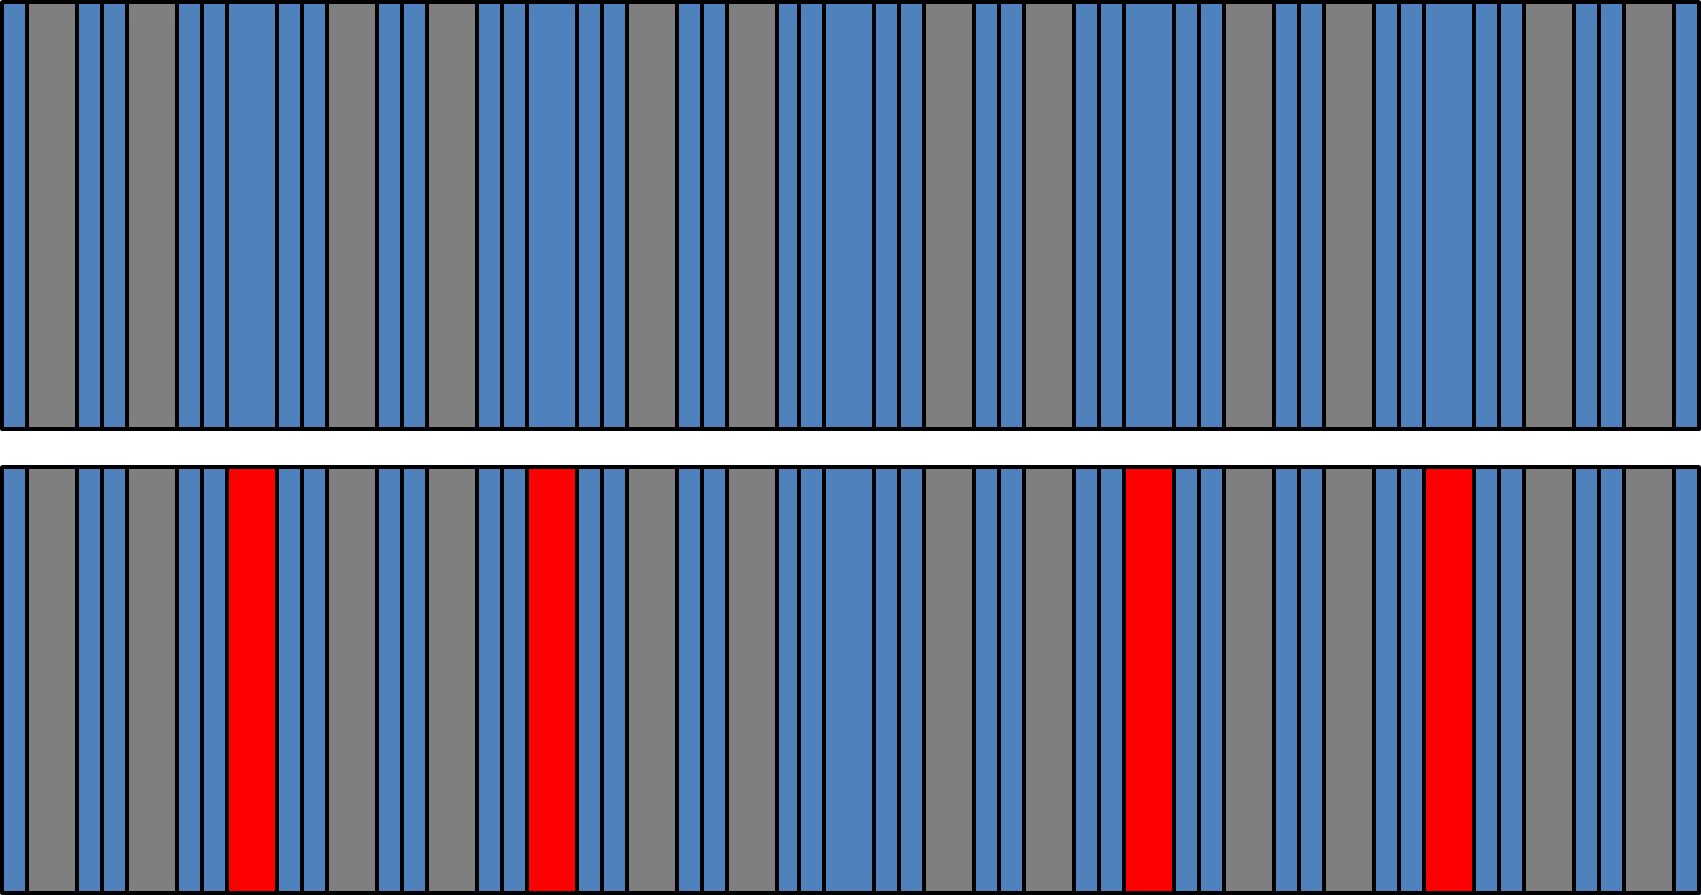
\includegraphics[width=\textwidth]{1dmoc-3x17-geom.png}
    \caption[Illustration of 1D MOC Test Geometry]{Illustration of 1D MOC 3$\times$17 geometry, where the top part represents the left and right assemblies and the bottom part represents the center assembly, with materials fuel (grey), control rod/moderator mixture (red), and moderator (blue)}\label{f:1dmoc-17x17-geom}
\end{figure}

The problem used for these calculations was a 1D variation of VERA Problem 4, illustrated in Figure \ref{f:1dmoc-17x17-geom}.  The center row of pins across all three assemblies was pulled out and used for the 1D model, resulting in a row of 51 pins (17 pins across, 3 assemblies) with a pin pitch of 1.26 cm (the inter-assembly gap was neglected for this model).  The center assembly had 4 guide tubes in it which contained a mixture of moderator and control rod to represent a partially inserted control rod.  These partially rodded locations were the only part of the problem that had any material changes.  This allowed the effects of the cross-section homogenization to be isolated for each calculations.

\subsection{1D MOC Investigation}

\subsubsection{Specified Total Source}

The first set of calculations performed were done using a specified total source.  To do this, the guide tubes were filled with 50\% control rod and 50\% moderator volume fraction mixture, and a full eigenvalue calculation was performed.  The total source distribution (fission and scattering) from this calculation were then passed to the the fixed source solver.  A single iteration was run using this source on three different variations of the problem: the 50-50 mixture, fully rodded, and fully unrodded.  Because the multi-group source is set up before performing any MOC sweeps, this resulted in all three of those calculations having an identical source for the MOC sweep.  The only difference between them was the cross-sections used in the guide tubes.

Figure \ref{f:1dmoc-fixed-50-scalflux7} shows the scalar flux resulting from these three calculations.  The most important thing to note in this data is that the effects of the rod are very local in the MOC calculation.  Moving through the rodded pin cell, the rodded, unrodded, and mixed cases have converged back to the same shape by the time the edge of the partially rodded pin cell is reached.  Because of the exponential nature of the MOC solution in equation \hl{number}, if the sources are the same the two different solutions converge to each other quickly as you move away from the rod.

\begin{figure}[H]
    \centering
    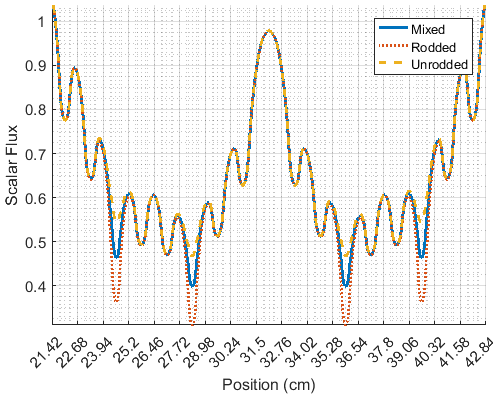
\includegraphics[width=0.7\textwidth]{1dmoc-50mix-fixedscat-scalflux7.png}
    \caption{Group 7 scalar flux comparisons for a fixed fission and scattering source calculation}\label{f:1dmoc-fixed-50-scalflux7}
\end{figure}

Figure \ref{f:1dmoc-fixed-50-angflux} shows the right-going angular flux in groups 1 (fast) and group 7 (thermal) for the center assembly.  The group 7 angular flux behaves similarly to the group 7 scalar flux in that the effects are localized around each rod.  The three different angular flux shapes are still somewhat different at the edge of the neighboring pin cell, but these differences are nearly indiscernible upon reaching the clad and fuel in the next pin cell.  The reason for this is that the mean free path of thermal neutrons is small.  The total group 7 cross-section in the moderator is about 2.65 cm$^{-1}$, which corresponds to a mean free path of about 0.38 cm, which is less than one third of the pin pitch for a typical PWR.  This combined with the exponential behavior of the MOC solution washes out the differences between the solutions quickly upon moving away from the rodded region.

\begin{figure}[H]
    \centering
    \subfigure[Group 1]{
        \centering
        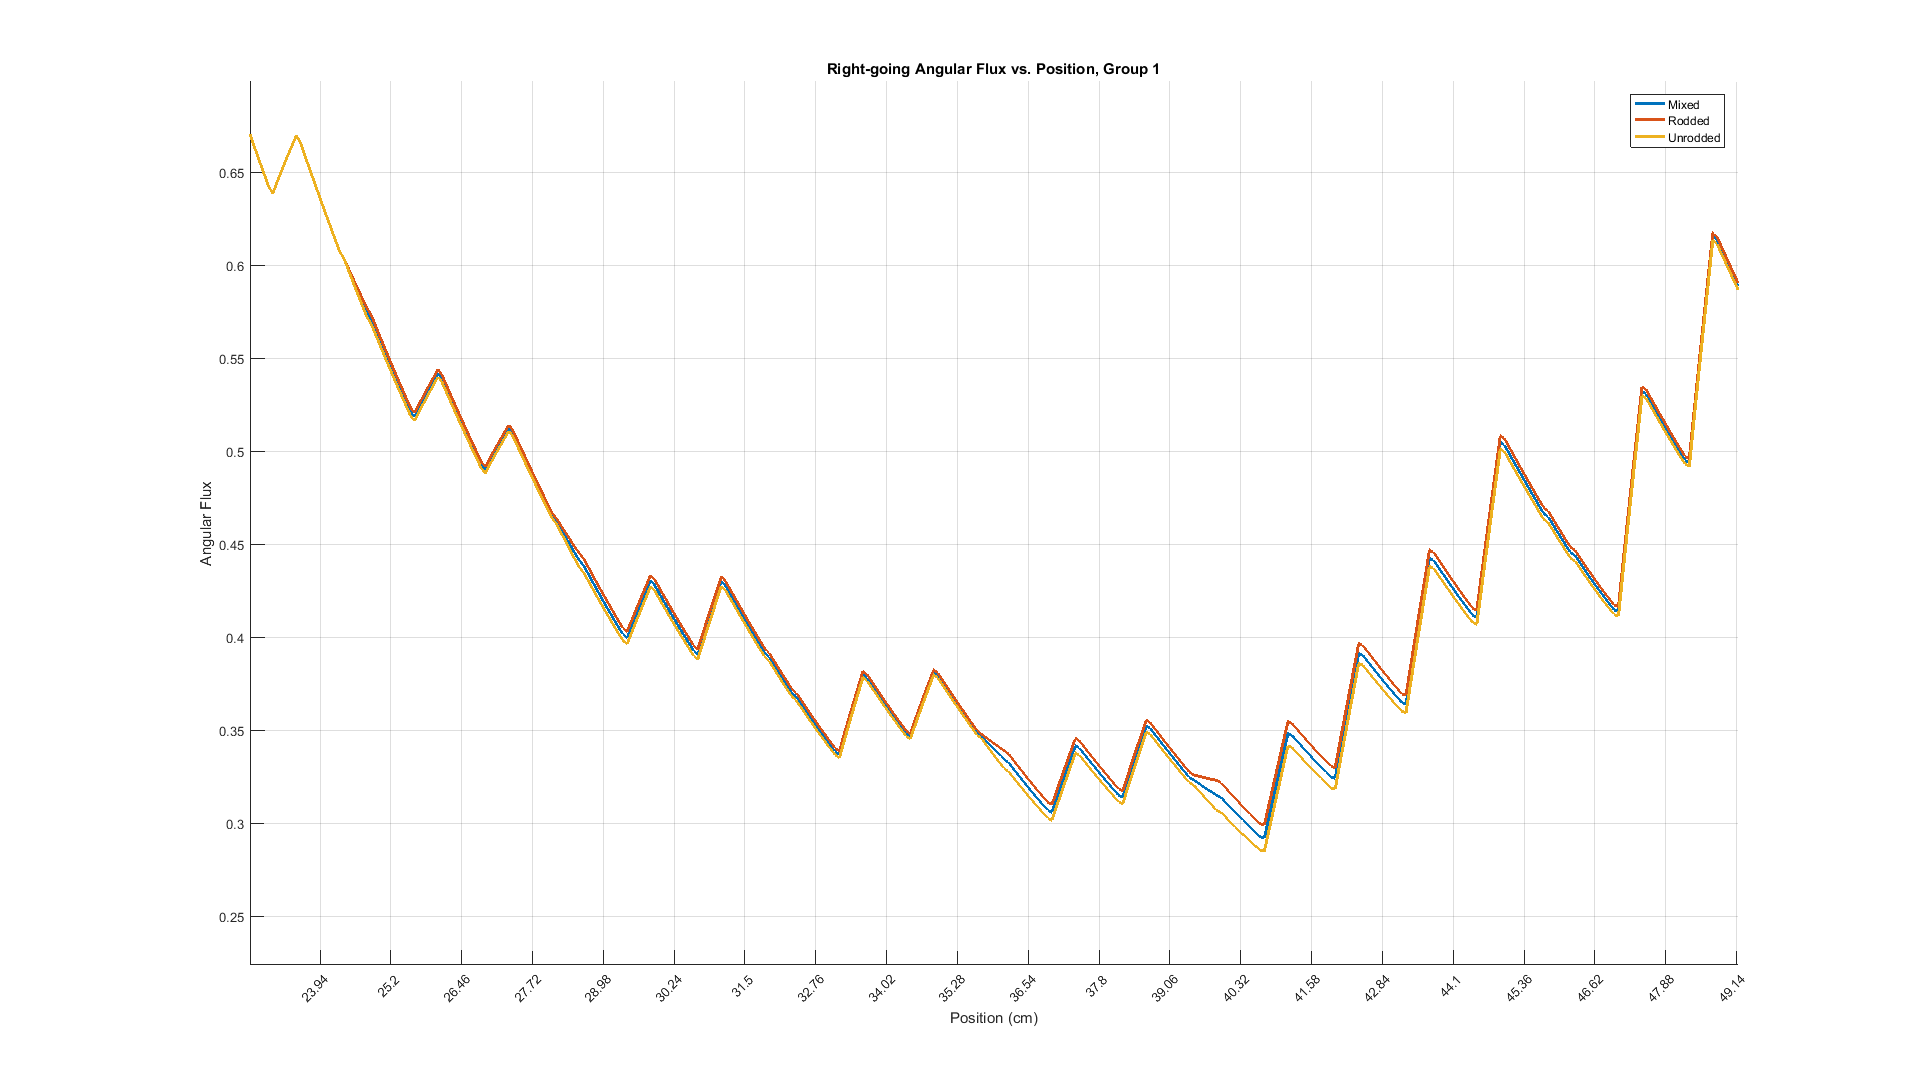
\includegraphics[width=0.45\textwidth]{1dmoc-50mix-fixedscat-angflux1.png}
        \label{f:1dmoc-fixed-50-angflux1}
    }
    \hfill
    \subfigure[Group 7]{
        \centering
        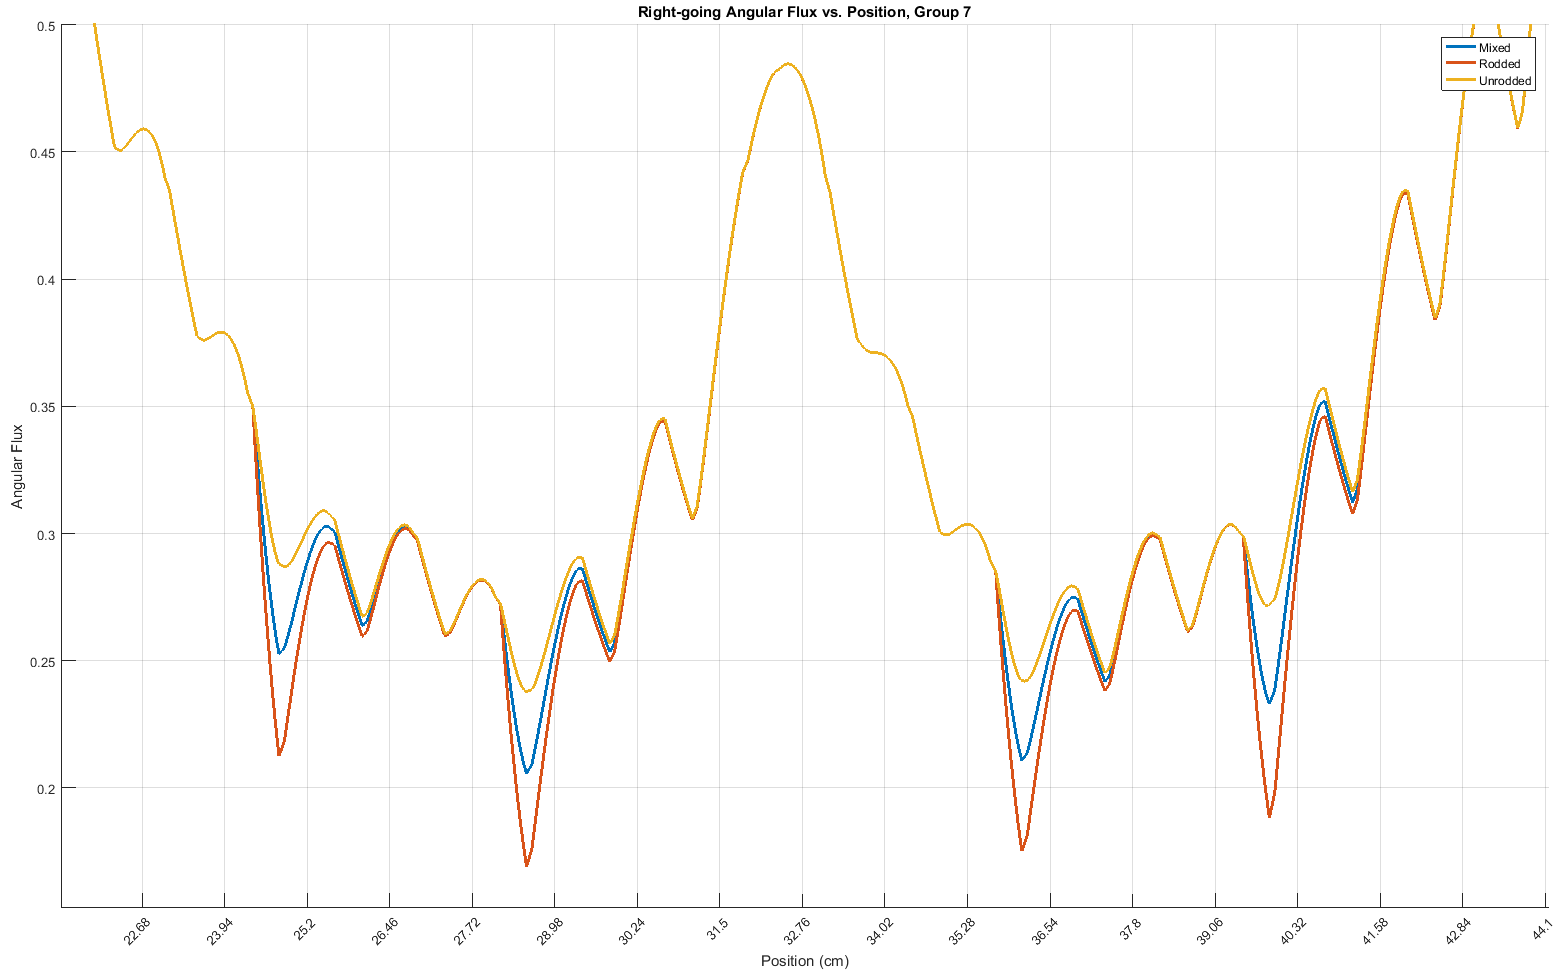
\includegraphics[width=0.45\textwidth]{1dmoc-50mix-fixedscat-angflux7.png}
        \label{f:1dmoc-fixed-50-angflux7}
    }
    \caption{Angular flux comparisons for a fixed fission and scattering source calculation}\label{f:1dmoc-fixed-50-angflux}
\end{figure}

The same cannot be said for the fast flux.  The mean free path of the fast flux is about 6.3 cm, which is the width of five pin cells.  Thus, it can be seen that each of the control rods after the first builds on the effects of the previous control rod.  Thus, the largest differences between the solutions is seen near the exit of the assembly after passing through all 4 rodded regions.  However, the differences are still small since control rods are generally thermal absorbers and have only a small impact on the flux in fast energy groups.

\subsubsection{Fixed Fission Source}

\begin{figure}[H]
    \centering
    \subfigure[25\% Mixture]{
        \centering
        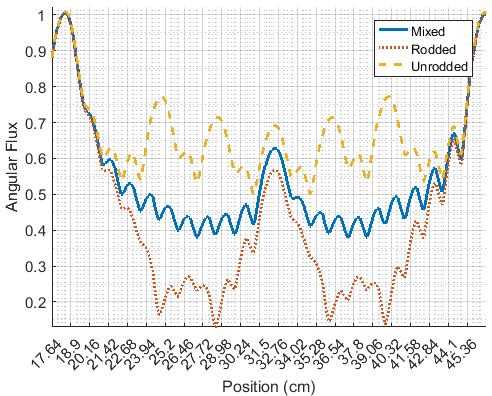
\includegraphics[width=0.45\textwidth]{1dmoc-25mix-angflux7.png}
        \label{f:1dmoc-25-angflux7}
    }
    \hfill
    \subfigure[50\% Mixture]{
        \centering
        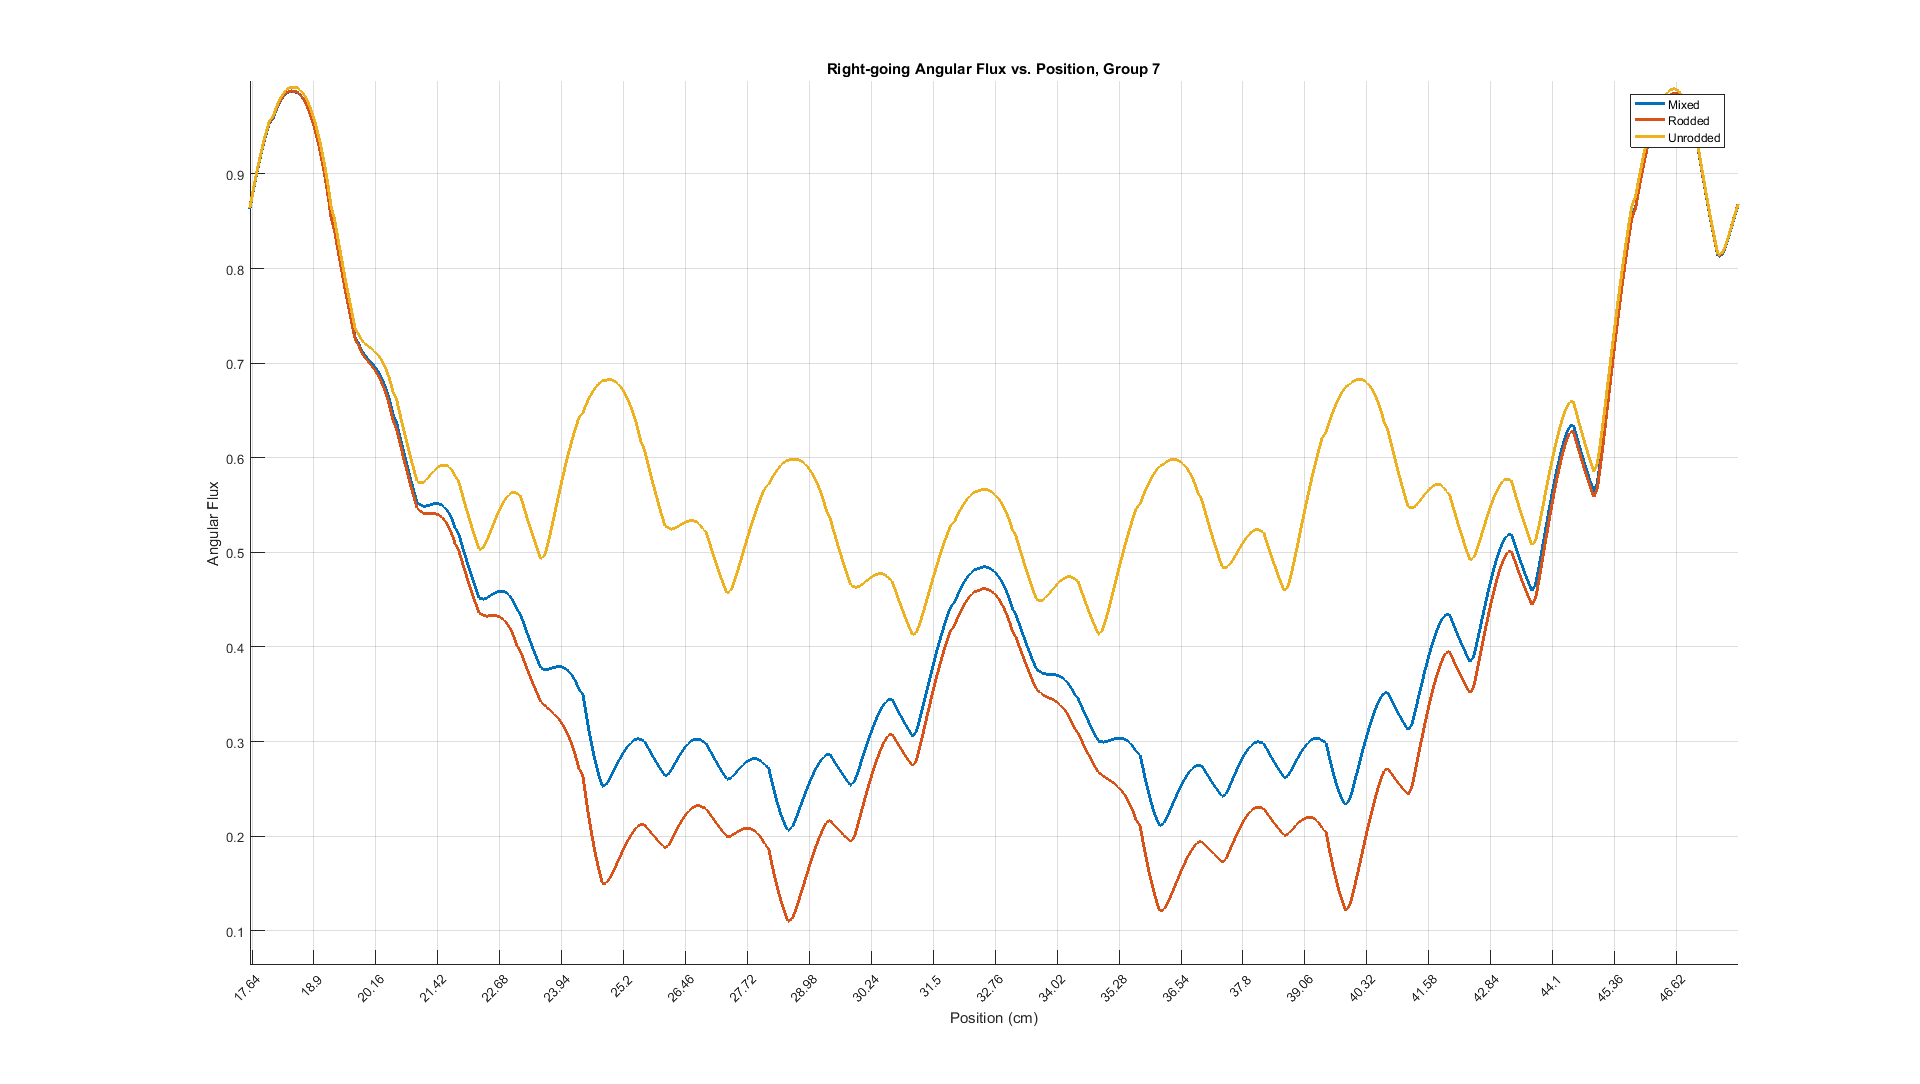
\includegraphics[width=0.45\textwidth]{1dmoc-50mix-angflux7.png}
        \label{f:1dmoc-50-angflux7}
    }
    ~
    \subfigure[75\% Mixture]{
        \centering
        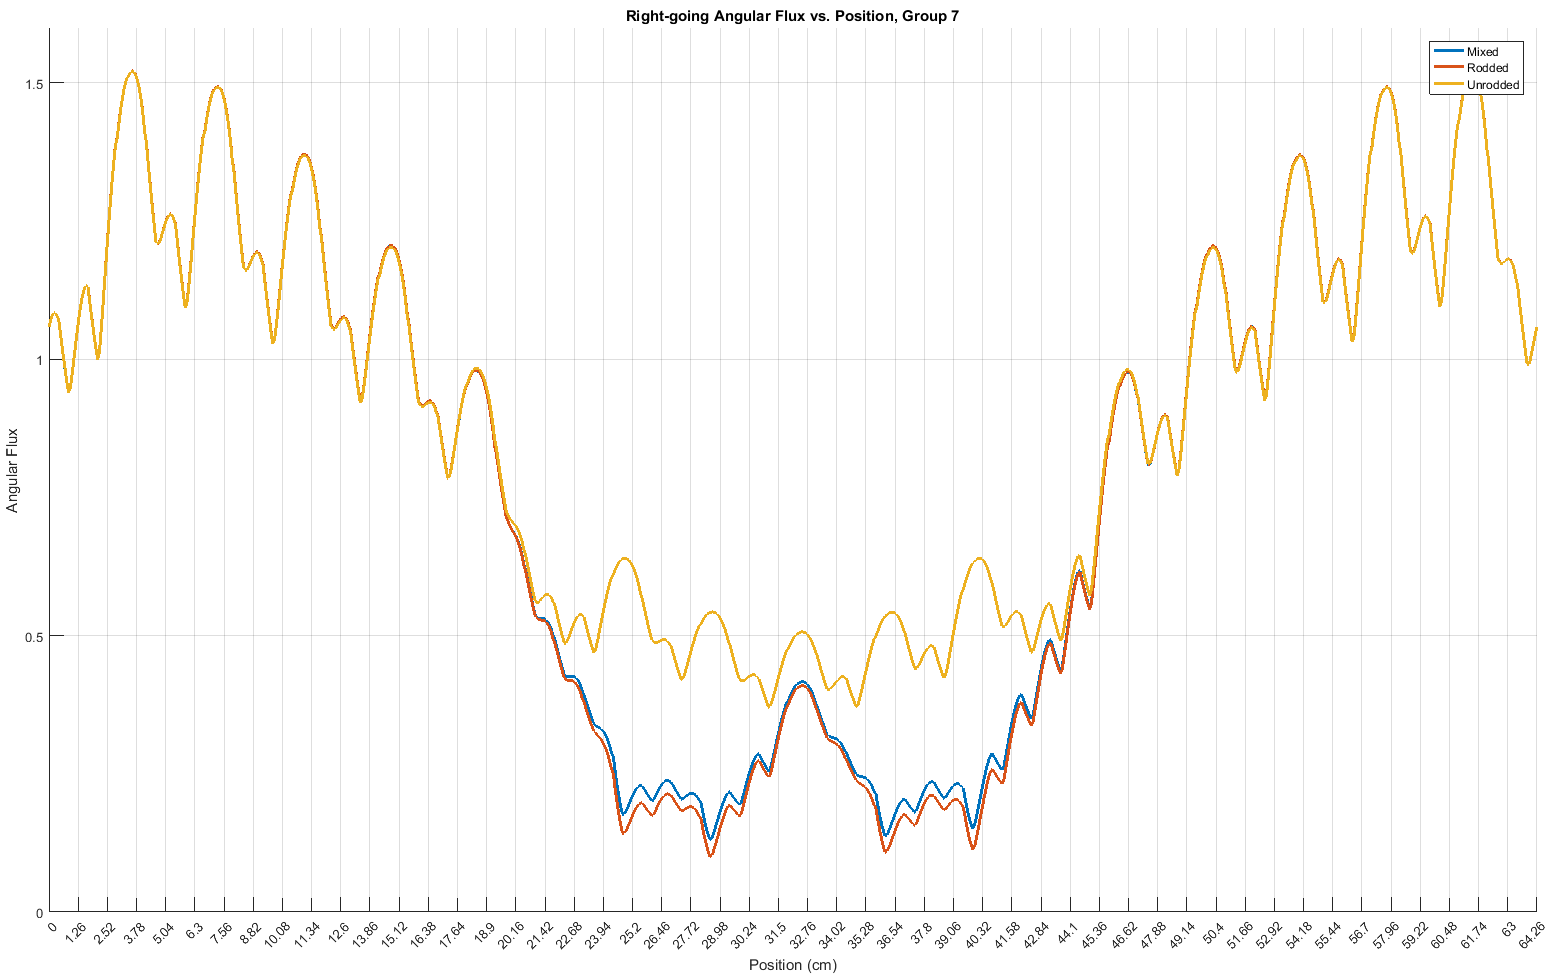
\includegraphics[width=0.45\textwidth]{1dmoc-75mix-angflux7.png}
        \label{f:1dmoc-75-angflux7}
    }
    \caption{Group 7 angular flux comparisons for 25\% and 75\% mixtures}\label{f:1dmoc-angflux7}
\end{figure}

The second set of calculations that was performed used a fixed fission source, but allowed the scattering source to fully converge for each calculation.  As in the previous section, an eigenvalue calculation was completed using partially rodded cross-sections.  This was done for 25\%, 50\%, and 75\% rodded cases.  For each case, a fixed fission source calculation was done with the fully rodded and fully unrodded cross-sections.  This time, multiple iterations were allowed for each material to converge the scattering source.  This allows us to see the effects of the rod on the scattering source distribution without worrying about changes in the eigenvalue and fission source distribution.

\begin{figure}[H]
    \centering
    \subfigure[25\% Mixture]{
        \centering
        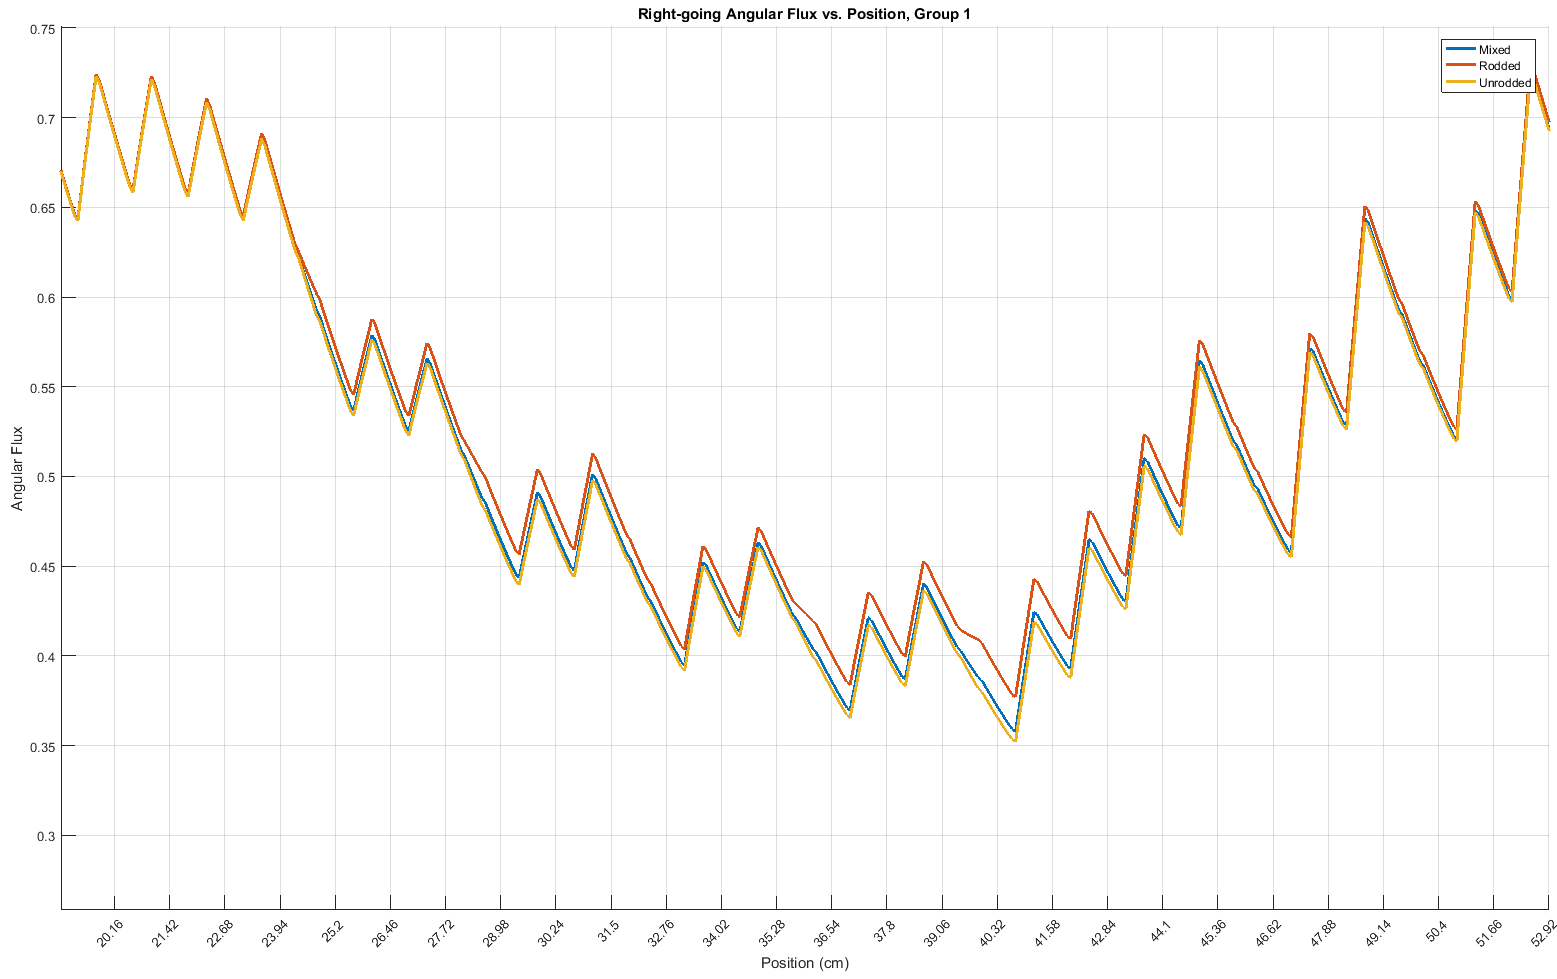
\includegraphics[width=0.45\textwidth]{1dmoc-25mix-angflux1.png}
        \label{f:1dmoc-25-angflux1}
    }
    \hfill
    \subfigure[50\% Mixture]{
        \centering
        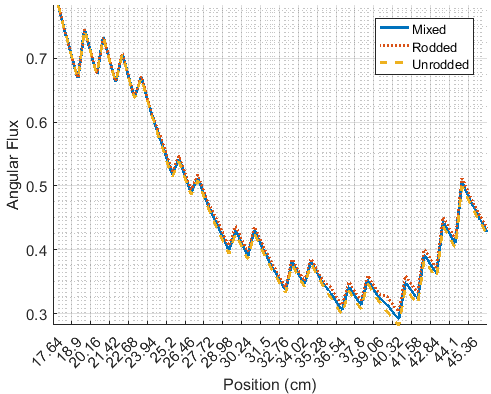
\includegraphics[width=0.45\textwidth]{1dmoc-50mix-angflux1.png}
        \label{f:1dmoc-50-angflux1}
    }
    ~
    \subfigure[75\% Mixture]{
        \centering
        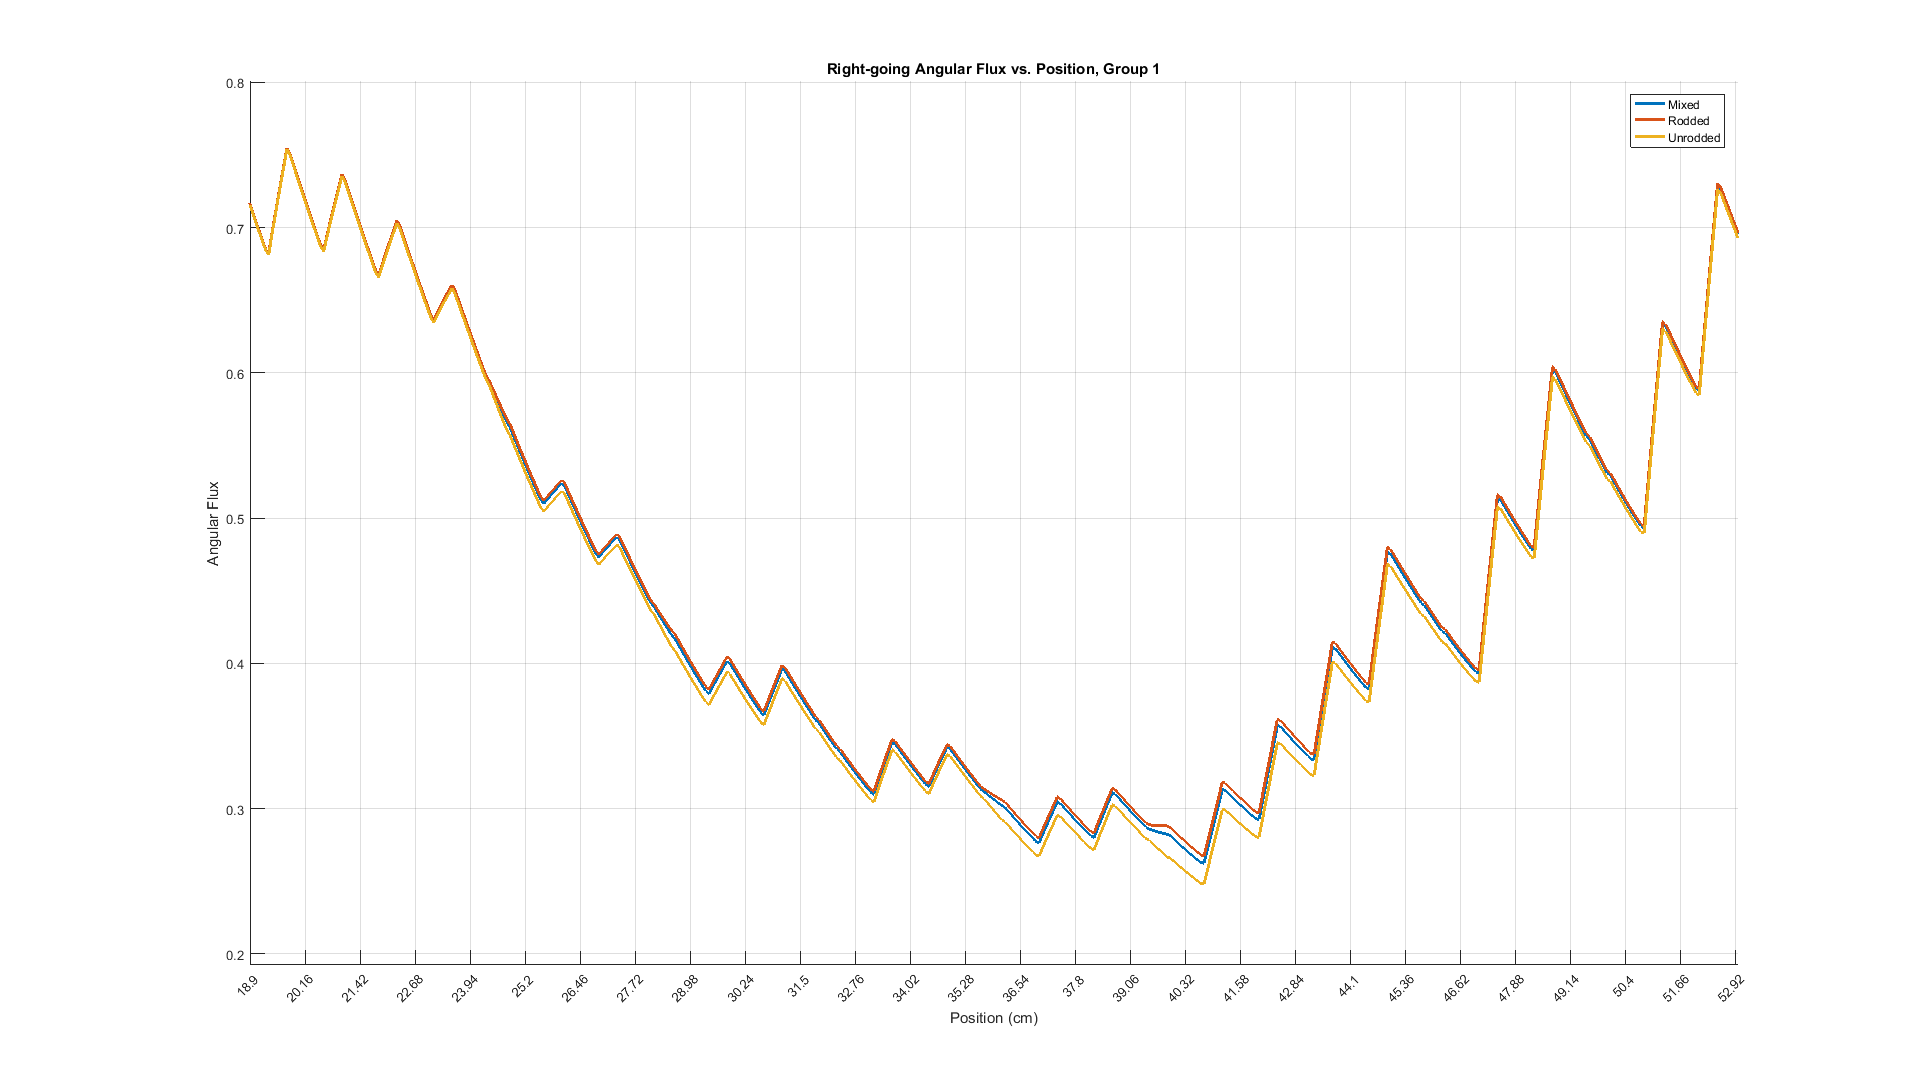
\includegraphics[width=0.45\textwidth]{1dmoc-75mix-angflux1.png}
        \label{f:1dmoc-75-angflux1}
    }
    \caption{Group 1 angular flux comparisons for 25\% and 75\% mixtures}\label{f:1dmoc-angflux1}
\end{figure}


Figure \ref{f:1dmoc-angflux7} shows the group 7 angular flux comparisons for each of the three mixtures.  We immediately see that for each of them, the angular flux for the mixture is skewed toward the rodded result instead of being a volume-fraction--weighted average of the rodded and unrodded solutions.  For example, comparing Figures \ref{f:1dmoc-50-angflux7} and \ref{f:1dmoc-fixed-50-angflux7} shows that the angular flux is much closer to the rodded solution than when the scattering source was fixed, despite the small mean free path of thermal neutrons.  Figure \ref{f:1dmoc-angflux1} shows the same comparison for the fast flux and provides some insight into the differences in the thermal flux solutions.  The difference between the rodded, unrodded, and mixed fast fluxes are small for this calculation, similarly to the fixed total source calculations in the previous section.  However, these small differences have the effect of spreading the scattering source across the problem due to the long mean free path.  Thus, the small differences in the fast flux cause large differences in the thermal flux scattering source, which in turns effects the fission source throughout the problem.

It should be noted as well that all angular flux plots shown here are for the flattest polar angle.  Since the steeper angles travel through more material in each region, the differences between them go away more quickly.  However, as long as some angles are flat, these effects on the source will be seen throughout the problem domain.

\subsubsection{Summary}

These calculations provide several insights into what a new decusping method must be able to accomplish.  First, it must be able to account for the heterogeneous rodded and unrodded cross sections.  This is critical to obtaining an accurate shape for the thermal flux.  Second, sources must be calculated around the partially inserted rod using different scalar fluxes.  If the same scalar flux is used for both the rodded and unrodded calculations, the results are non-sensical.  Finally, the angular flux exiting the partially rodded region must accurately represent the partially inserted rod, especially for the fast flux.  If this outgoing flux is skewed incorrectly toward the rodded or unrodded fast flux solution, even small errors can have a significant impact on the scattering and fission source distributions throughout the rest of the problem.

\subsection{Subray MOC Description}

Using the results of the 1D MOC investigation described above, a new method has been developed called the subray methods of characteristics, illustrated in Figure \ref{f:subrayMOC}.  For the majority of a domain, this method will behave the same as traditional MOC.  However, when approaching a region with a partially inserted rod, the ray along which the angular flux is being solved can be split into two (or more) separate rays.  One ray will use the control rod cross section while the other will use the cross section for the material below the control rod.  In each region where subray MOC is used, the scalar flux can be tallied using a modified form of equation \hl{number}:
\begin{equation}
stuff
\end{equation}
This equation averages the angular flux for each subray segment to obtain an axially-averaged, segment-averaged angular flux, which is then used to calculate the scalar flux.  Furthermore, the subray angular fluxes can also be used to calculate the scalar flux for these subregions to generate subregion source terms for the subsequent iteration.

After passing completely through the partially rodded regions, the subray angular fluxes can be recombined into a single ray using the volume fractions associated with each subray.  The errors introduced from this are minimal do to the exponential nature of the MOC ray calculations.  After the rod, both subrays have the same cross section again and the axial shape of the sources begins to flatten out.  Based on equation \hl{number}, the rays then exponentially converge toward each other.  Thus, as long as an appropriate amount of distance is left between the end of the partially rodded region and the recombination point, minimal errors are introduced.  This is discussed in more detail in section \hl{number}.

\begin{figure}
    \centering
    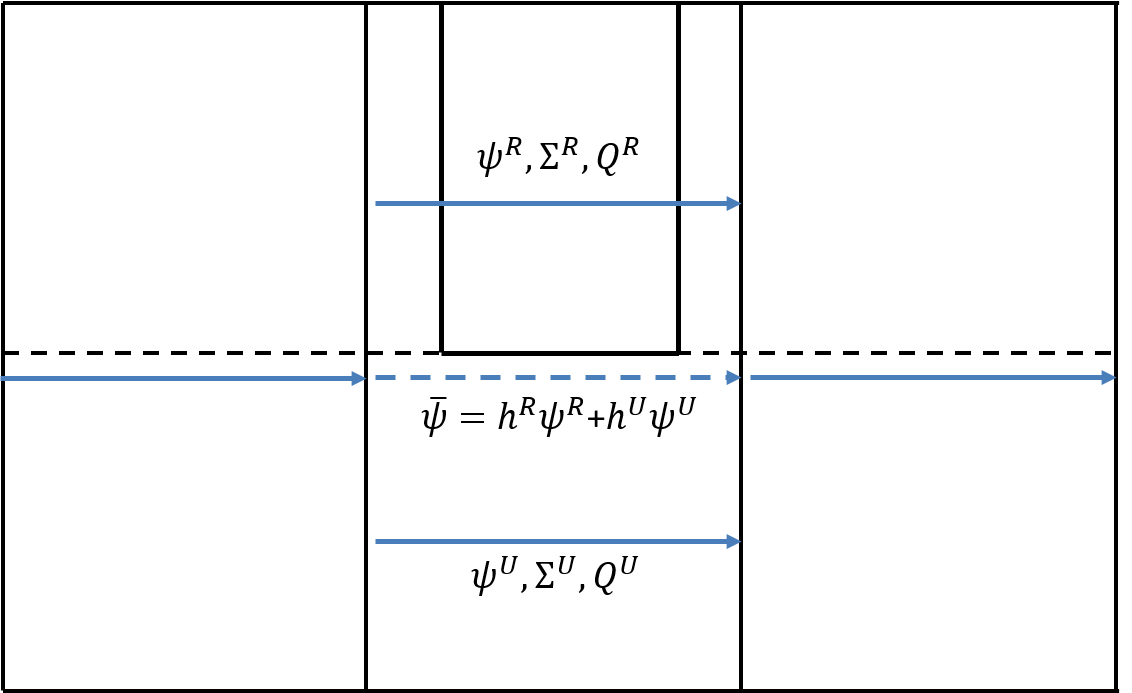
\includegraphics[width=0.8\textwidth]{sub-ray_illustration.png}
    \caption{Illustration of subray method of characteristics for partially inserted rod}\label{f:subrayMOC}
\end{figure}

This method should accurately capture the cross section and source effects around the partially inserted rod by using subrays.  Furthermore, recombining the outgoing fluxes after the rod should provide a more accurate outgoing flux than that calculated from a homogenized cross section.  This method addresses all the insights gathered from the 1D MOC investigation.  Furthermore, it addresses all the limitations of the polynomial and subplane collision probabilities decusping techniques discussed earlier in this chapter.

\subsection{MPACT Implementation}

Implementation of subray MOC in the 1D MOC code is straightforward since the code is small and uses only power iteration.  Implementing the method in the 2D/1D code MPACT is significantly more complicated.  First, even for single-plane 2D cases, MOC calculations can be expensive.  Because of this, the MOC sweep kernels need to be modified to use subray in such a way that the kernels will still be well optimized for the subray calculations.  When moving from 2D to 2D/1D other complexities are introduced from the 3D CMFD and 1D P$_3$ calculations that have to be correctly incorporated in the subray MOC calculations.  The following sections discuss some of the details of how this is done.

\subsubsection{MOC Sweeper Modifications}

Implementing a subray MOC sweeper in MPACT presents some difficulties since MPACT was not designed with these types of subgrid methods in mind.  The MOC sweepers have been optimized to ensure that the rays are swept in the most efficient way possible.  The long rays are set up once up front, then they are swept in a separate loop with no branching statements to ensure the hardware is performing the calculations as quickly as possible.  Subray MOC naturally introduces branching statements that would destroy this efficiency.

To get around this, an extra loop was added just inside the loop over long rays.  This loop goes from one to the number of subrays for that long ray.  For most long rays, this number will just be one, meaning that long ray gets swept exactly one time.  The results of the sweep for those long rays is exactly the same as if subray MOC were not being used.  For the long rays that intersect with a partially rodded region, the ray is constructed and swept multiple times.  During the sweep, volume fractions are used to tally the surface currents for CMFD and the region-wise scalar fluxes outside the partially rodded region.  Inside the partially rodded region, the scalar fluxes are tallied into two separate regions (one rodded, one unrodded).  This allows these subregion scalar fluxes to construct the scattering source for the next iteration.  After the sweep of the full plane is complete, the subregion scalar fluxes are combined using volume fractions as a post-processing step.

This approach has the drawback of duplicating several of the long rays.  For problems discussed in chapter \hl{number}, we can reasonably expect around 20-30\% of the long rays to intersect a partially rodded region.  However, this approach allows the MOC sweeper kernels to maintain a high degree of efficiency during the calculations.  Furthermore, based on duplicating 30\% of the long rays, we could expect a 30-40\% speedup compared with simply having 2 separate MOC planes to resolve the partially inserted rod.  Thus, taking this approach allows subray MOC to be implemented and tested without rewriting MPACT while still attaining significant speedup.

\subsubsection{Subregion and Recombination Selection}

Before performing the subray MOC sweeps, it must be determined which long rays will be duplicated.  This is done by examining the mesh for partially rodded regions.  Due to the source effects described in section \hl{number}, whenever a partially rodded region is identified, all other regions in that pin cell are also flagged as partially rodded.  This allows the axial shape of the source in the surrounding moderator region to also be resolved.

\begin{figure}
    \centering
    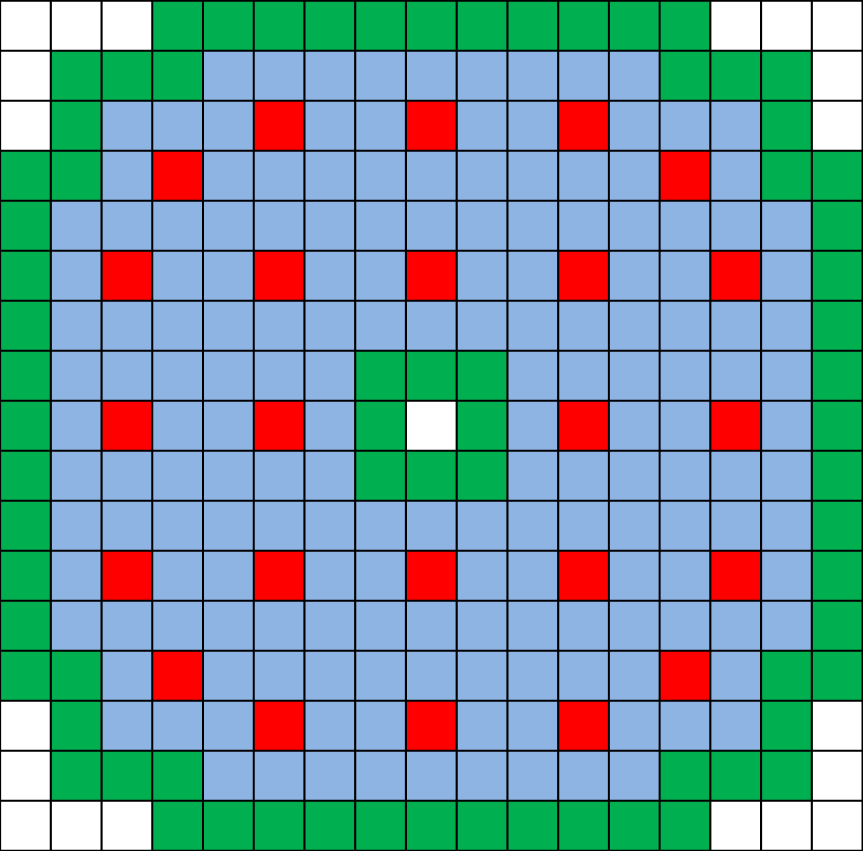
\includegraphics[width=0.8\textwidth]{recombination.png}
    \caption{Illustration of subray MOC regions selection process for a 17$\times$17 assembly for recombination factors of 0 (red), 1 (blue), 2 (green), and 3 (white).}\label{f:recombination}
\end{figure}

After identifying these regions, neighboring pins can also be flagged.  As more rings of neighboring pins are added, the solution should grow closer to that of 2 separate MOC planes.  In MPACT, this was implemented via a user-defined recombination flag.  A value of 0 will only mark partially rodded regions; a value greater than 0 will add that number of rings around the partially rodded pin cell.  Once all these regions are identified, any long ray that passes through any of these regions will be swept multiple times using subray MOC.  Some of these rays will not actually intersect the control rod at all, but will serve to resolve the source effects surrounding the rods.  The rays will ``split'' upon entering any of the flagged regions and will recombine only upon entering a non-flagged region.  In Figure \ref{f:recombination}, a recombination value of 0 will use subray only for the red pins, which actually have partially inserted control rods; a value of 1 will use subray for red and blue pins; a value of 2 will use subray for red, blue, and green pins; and a value of 3 will use subray for the entire assembly.  Regardless of the value, regions in neighboring assemblies will not be flagged unless those assemblies also have partially inserted control rods.

\subsubsection{Subplane CMFD and \texorpdfstring{P$_3$}{P3}}

Another consideration that must be made is that of the subplane scheme and its interactions with subray MOC.  While subray MOC could conceivably be used without the subplane scheme, having subplane should greatly improve its usefulness.  When projecting the CMFD solution back to the MOC mesh, the MOC fluxes are scaled by averaging the CMFD fluxes over the full height of the MOC plane, as discussed in section \hl{number}.  However, because the subplane CMFD solution has subgrid data, it can also be used to scale the subregion scalar fluxes from the subray MOC calculation, improving the accuracy and convergence of the subregion scattering and fission sources used for subray MOC.

Furthermore, the axial P$_3$ calculations are also done on the subplane scheme.  The regular MOC regions will use currents at the top and bottom of the MOC plane to calculate the axial TL source.  If the subplanes are aligned with the control rod, then currents are also available at the top and bottom of each of the subregions used by subray MOC.  This allows a more accurate axial shape for the axial TL source, which cahnges especially quickly in the vicinity of a control rod tip.  Thus, using the subplane scheme will greatly improve the accuracy of all three sources used by MOC in the 2D/1D method: scattering, fission, and axial TL.

One final consideration that must be made for subplane CMFD and subray MOC is that of the radial $\hat{D}$ terms.  Normally, the radial coupling coefficients should be calculated on the full-height MOC plane and applied to all subplanes belonging to that plane.  This is necessary because consistency between the diffusion and trasnport solutions needs to be enforced on the transport mesh.  However, when using subray MOC, surfaces which neighbor subregions will have their currents tallied on the subplane mesh, while other surfaces have their currents tallied on the MOC mesh.  When setting up the CMFD matrix, $\hat{D}$ terms on surfaces next to subregions should be calculated using currents for each of the subplanes, while the remaining $\hat{D}$ terms should be calculated using average currents from the full-height MOC plane.  This ensures the greatest accuracy and stability during the 2D/1D iteration when using subray MOC.

\section{Summary}

This chapter presented 3 new rod decusping techniques for the 2D/1D method.  These techniques vary in complexity and expected accuracy, but each of them captures some of the effects of the partially inserted control rod.  The following chapter will present the results of calculations using each of these methods and provide futher discussion on the strengths and limitations of each method.